\section{System Architecture}
\label{sec:system_architecture}
\subsection{Hardware Core System Block Diagram}
\begin{figure}[H]
	\centering
	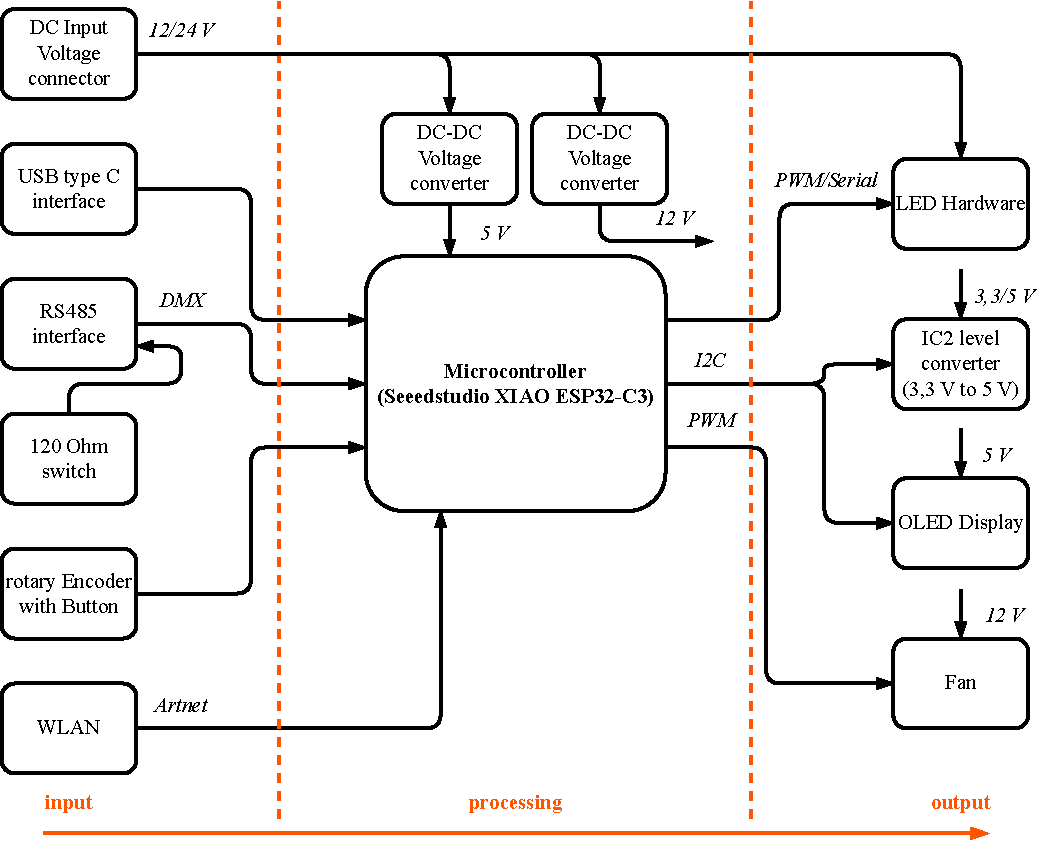
\includegraphics[width=0.95\linewidth]{graphics/hardware_architecture}
	\caption{Hardware System Architecture}
	\label{fig:hardwarearchitecture}
\end{figure}
The hardware architecture of the developed embedded \ac{LED} controller is segmented into three primary functional blocks: input, processing, and output. This design facilitates modularity and clear separation of concerns within the system. The schematic representation of this architecture can be seen in the provided diagram.

\subsubsection*{Input Block}

The input block is responsible for receiving power, data, and user commands.

\begin{itemize}
	\item \textbf{Power Supply:} The system accepts a flexible \ac{DC} input voltage ranging from 12V to 24V via a dedicated connector. This allows for compatibility with common power supplies found in lighting applications.
	\item \textbf{Programming and Debugging:} A \ac{USB} Type C interface is incorporated for firmware flashing, debugging, and potential serial communication during development.
	\item \textbf{Wired Communication:} An \ac{RS485} interface enables robust, long-distance wired communication, commonly used for protocols like \ac{DMX} in lighting control. A notable feature is an integrated switch to engage or disengage a 120 Ohm termination resistor, crucial for maintaining signal integrity in \ac{RS485} networks.
	\item \textbf{User Interface:} Direct user interaction is managed by a rotary encoder equipped with a push-button function. This allows users to navigate menus displayed on the \ac{HMI} and confirm selections.
	\item \textbf{Wireless Communication:} The controller integrates a 2.4 GHz \ac{WLAN} interface, enabling it to connect to standard wireless networks. This facilitates wireless control primarily through the Artnet protocol, a common standard for transmitting \ac{DMX} data over Ethernet networks.
\end{itemize}

\subsubsection*{Processing Block}

The processing block handles power regulation and executes the core logic of the controller.

\begin{itemize}
	\item \textbf{Power Conversion:} An essential component is the 5V DC-DC converter. This module steps down the incoming 12/24V supply to a regulated 5V. This stable 5V rail powers the sensitive electronic components, including the microcontroller and the display. \\
	For the spotlight a DC-DC converter provides a 12 V power rail. In this case, the input voltage does not match the fan voltage and is therefore needed. 
	\item \textbf{\ac{MCU}:} The central processing unit is the Seeedstudio XIAO ESP32-C3 microcontroller. This \ac{MCU} was chosen for its integrated Wi-Fi capabilities, sufficient processing power for handling communication protocols and control algorithms, and its compact form factor. It executes the firmware that manages inputs, processes control data (e.g., Artnet, \ac{DMX}), and drives the outputs.
\end{itemize}

\subsubsection*{Output Block}

The output block interfaces with the external components that the controller manages.

\begin{itemize}
	\item \textbf{\ac{LED} Control:} The primary function is controlling \ac{LED} hardware. The system is designed to support two main methods: direct serial communication for addressable \ac{LED} strips and \ac{PWM} control for driving different color channels (e.g., \ac{RGB}) of non-addressable \ac{LED}s.
	\item \textbf{Display Interface:} An \ac{I2C} interface is utilized to communicate with the \ac{OLED} display, which serves as the \ac{HMI}. In certain product configurations, such as integrated panel lights, this \ac{I2C} bus may also be used to send control data to other integrated components. An \ac{I2C} level converter is included to shift voltage levels between the 3.3V logic of the \ac{MCU} and the 5V requirement of the other peripherals. The display works with either 3.3V logic or 5V. To only drive the display, the level converter is not needed.
	\item \textbf{Thermal Management:} To ensure reliable operation, the controller incorporates fan control via a standard \ac{PWM} interface, compatible with typical computer fans. This allows the system to regulate its temperature under load.
\end{itemize}

\subsection{Hardware Configuration Options}
While the core architecture remains consistent, different hardware configurations and \ac{PCB}s are available to suit various application requirements:

\begin{itemize}
	\item \textbf{Tube Light V2 (Non-Addressable \ac{LED}s):} This variant utilizes hardware supporting three \ac{PWM} outputs for controlling non-addressable \ac{LED} strips. It omits the fan control output as it's not typically required for this configuration.
	\item \textbf{Tube Light V3 (Addressable \ac{LED}s):} For tube lights using addressable \ac{LED}s, the hardware provides support for a serial data output. Similar to the non-addressable version, fan control is not included.
	\item \textbf{Panel Light:} This configuration uses the same fundamental hardware as the addressable \ac{LED} tube light (serial output capable). However, the \ac{RGB} data for the panel is specifically transmitted via the \ac{I2C} interface instead of the dedicated serial \ac{LED} output. This version includes the hardware connection for fan control.
	\item \textbf{Spot Light:} The spot light employs an individual \ac{PCB} design tailored to its needs. It features three \ac{PWM} outputs for \ac{LED} control and includes the hardware connection for fan control.
	The size of the \ac{PCB} is designed to fit within the casing. The previous \ac{PCB} would not fit.
\end{itemize}

These variations ensure that each product type has an optimized hardware platform based on the core controller design, omitting unnecessary components or adapting interfaces as needed for the specific application.

\subsection{Software Architecture for Multi-Configuration Support}
\subsubsection{Interfaces between software modules}
The software is structured around a central main.cpp file as seen in figure \ref{fig:softwareinterfaces}. 
Interactions between various hardware abstractions and logic modules are orchestrated there.
\begin{figure}[H]
	\centering
	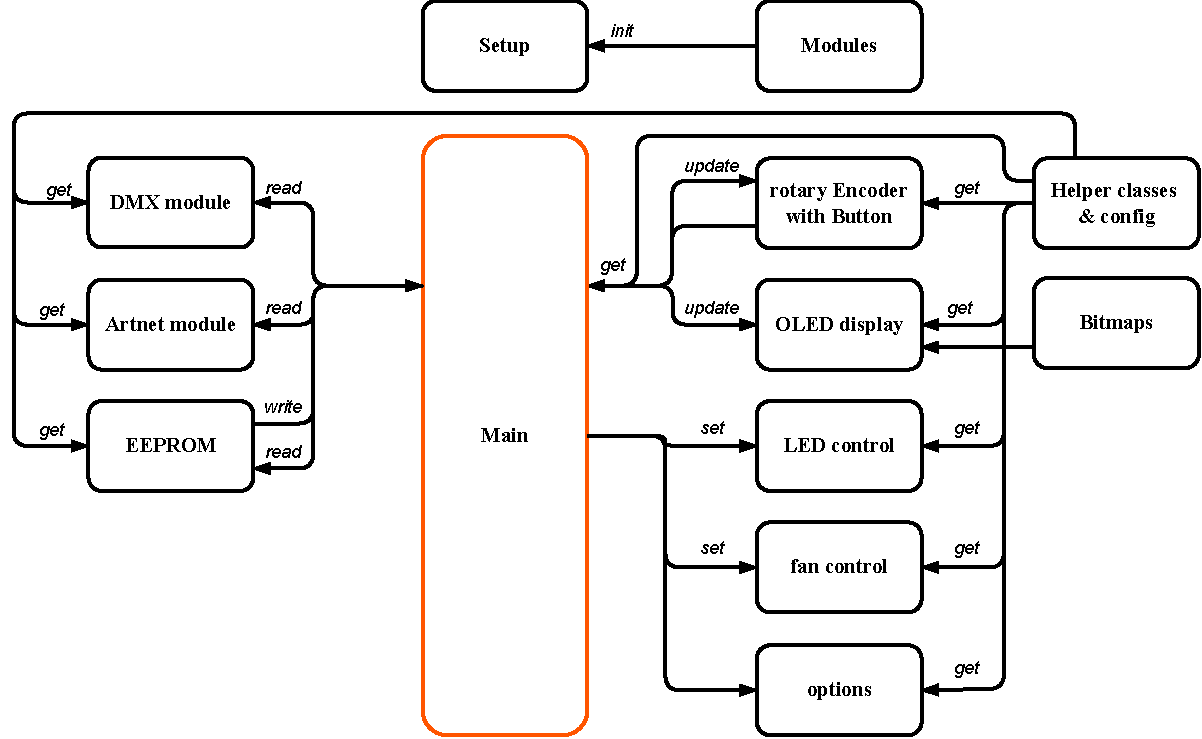
\includegraphics[width=0.95\linewidth]{graphics/software_interfaces}
	\caption{Interfaces of the software modules}
	\label{fig:softwareinterfaces}
\end{figure}
The software architecture features a central \texttt{Main} module (\texttt{main.cpp}) that coordinates interactions between several specialized modules. During startup, \texttt{Setup} initializes all other modules, including those managing hardware inputs (like the \texttt{Rotary Encoder}), outputs (\texttt{OLED Display}, \texttt{LED Control}, \texttt{Fan Control}), communication (\texttt{DMX Module}, \texttt{Artnet Module}), and data persistence (\ac{EEPROM}). \\

In the main loop, the \texttt{Main} module continuously polls the \texttt{Rotary Encoder} for user input events using getter functions. Based on the application state and user input, \texttt{Main} sends commands to update the \texttt{OLED Display} and control the \ac{LED} outputs via their respective modules. If enabled, fan speed adjustments are communicated to the \texttt{Fan Control} module.\\

Communication data for \ac{DMX} and Artnet is handled through dedicated modules. \texttt{Main} periodically checks for incoming \ac{DMX} data and initiates Artnet data parsing, receiving Artnet packets via a callback mechanism. Configuration and status information are exchanged using getter and setter methods provided by these communication modules.\\

Persistent storage of configuration settings is managed by the \ac{EEPROM} module, which provides interfaces for reading and writing the state of core application objects upon request from \texttt{Main}. Shared configuration values and helper classes containing state information are accessed by various modules as needed, typically through getter and setter methods.\\

\subsubsection{Main Loop}
The firmware executed by the \ac{MCU} operates based on a main execution loop, which continuously performs a sequence of tasks to manage the controller's functions. This loop is structured to ensure timely polling of inputs, processing of user interactions, and handling of communication protocols. \\

Initially, the loop polls the current state of all relevant hardware modules and software components, gathering the latest information. Following the polling stage, user input from the rotary encoder's push button is processed; the software distinguishes between short and long presses to enable different actions or menu navigation commands. Subsequently, changes in the rotary encoder's value are handled, typically translating these changes into menu navigation or parameter adjustments within the \ac{HMI}. \\

The loop then manages the state of the \ac{OLED} display, including standby or sleep modes, and updates the fan speed via \ac{PWM} based on thermal requirements or configuration (where applicable). Finally, several tasks are handled periodically within the loop's cycle. These include checking for the arrival of new \ac{DMX} data via the \ac{RS485} interface, managing the \ac{WLAN} connection for Artnet communication, and processing any received Artnet data packets. This structured, sequential, yet periodically interrupted approach ensures that all essential functions, from direct user interaction to network communication and output control, are managed efficiently within the controller's processing cycle.

\subsubsection{Menu Structure}
User interaction with the device primarily occurs through the rotary encoder and its integrated push button, as depicted in the menu structure diagram figure \ref{fig:menustructure}.
\begin{figure}[H]
	\centering
	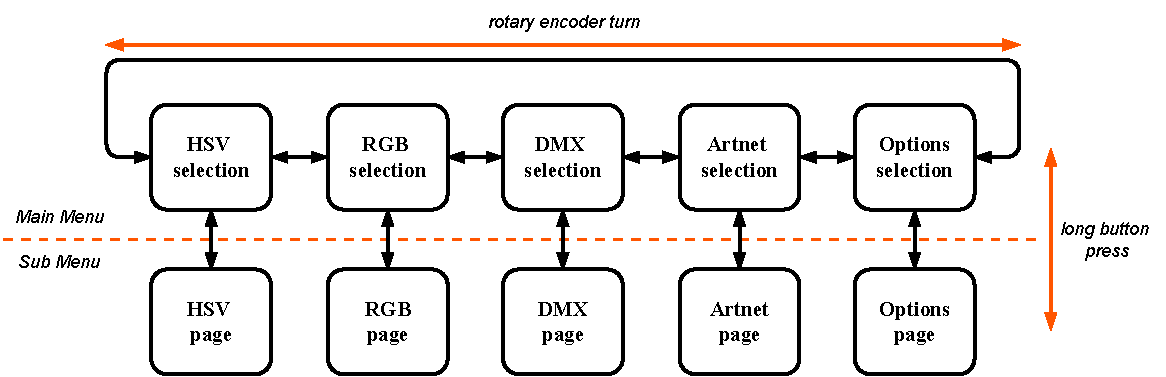
\includegraphics[width=0.95\linewidth]{graphics/menu_structure}
	\caption{Structure of the main menu navigation}
	\label{fig:menustructure}
\end{figure}

In the main menu view, turning the rotary encoder allows the user to cycle horizontally through the available function selections (such as \acs{HSV}, \ac{RGB}, \ac{DMX}, Artnet, and Options). The diagram confirms that this selection behavior includes wrap-around; if the user continues turning the encoder after reaching the first or last menu item, the selection jumps to the opposite end of the menu list, enabling continuous scrolling.\\

Vertical navigation between the main menu level and the corresponding submenu pages is achieved via a long press on the encoder's button. Performing a long press while a main menu item is selected transitions the software into that item's specific submenu, displaying its parameters or options. Conversely, performing another long press while within a submenu returns the user to the main menu selection screen. This hierarchical navigation, visually represented in the provided diagram, allows access to different functionalities and their settings using simple rotary and press actions.